\begin{figure}[H]
	\centering
	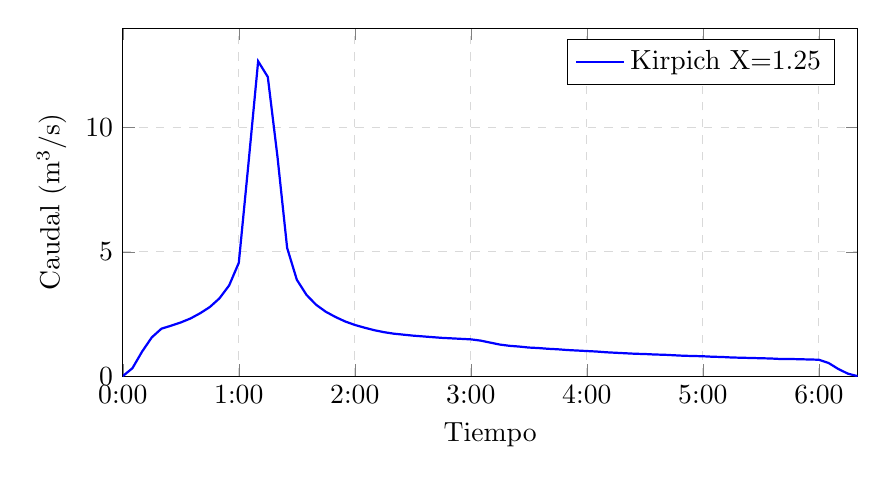
\begin{tikzpicture}
		\begin{axis}[
			width=0.9\textwidth,
			height=6cm,
			xlabel={Tiempo},
			ylabel={Caudal (m$^3$/s)},
			xmin=0,
			xmax=380,
			ymin=0,
			ymax=14,
			grid=major,
			grid style={dashed, gray!30},
			legend pos=north east,
			xtick={0, 60, 120, 180, 240, 300, 360},
			xticklabels={0:00, 1:00, 2:00, 3:00, 4:00, 5:00, 6:00},
			]
		% Kirpich X=1.25
		\addplot [
		blue,
		thick,
		solid,
		] coordinates {
				(0, 0.00) (5, 0.32) (10, 0.99) (15, 1.56) (20, 1.91)
				(25, 2.03) (30, 2.16) (35, 2.32) (40, 2.53) (45, 2.78)
				(50, 3.13) (55, 3.65) (60, 4.56) (65, 8.56) (70, 12.67)
				(75, 12.04) (80, 8.83) (85, 5.16) (90, 3.88) (95, 3.27)
				(100, 2.87) (105, 2.59) (110, 2.38) (115, 2.20) (120, 2.06)
				(125, 1.95) (130, 1.85) (135, 1.77) (140, 1.71) (145, 1.67)
				(150, 1.63) (155, 1.60) (160, 1.57) (165, 1.54) (170, 1.52)
				(175, 1.50) (180, 1.48) (185, 1.43) (190, 1.35) (195, 1.27)
				(200, 1.22) (205, 1.19) (210, 1.15) (215, 1.13) (220, 1.10)
				(225, 1.08) (230, 1.05) (235, 1.03) (240, 1.01) (245, 0.99)
				(250, 0.96) (255, 0.94) (260, 0.92) (265, 0.90) (270, 0.89)
				(275, 0.87) (280, 0.86) (285, 0.84) (290, 0.82) (295, 0.81)
				(300, 0.80) (305, 0.78) (310, 0.77) (315, 0.75) (320, 0.74)
				(325, 0.73) (330, 0.72) (335, 0.71) (340, 0.69) (345, 0.69)
				(350, 0.68) (355, 0.67) (360, 0.66) (365, 0.53) (370, 0.29)
				(375, 0.10) (380, 0.00)
		};
		\addlegendentry{Kirpich X=1.25}

		\end{axis}
	\end{tikzpicture}
	\caption{Hidrograma - Kirpich + GZ $T_r$=10 años ($Q_p$=12.672 m$^3$/s)}
	\label{fig:hydro_kirpich_gz_Tr10_X125}
\end{figure}
